\begin{frame}{Thực nghiệm - Phân loại cấu hình}
  \begin{figure}
    \centering
    \subfloat[Lớp C]{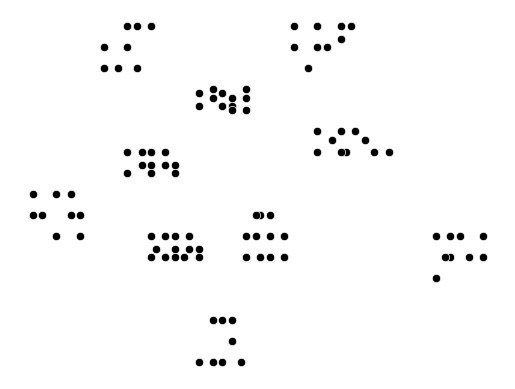
\includegraphics[width=0.3\linewidth]{figures/cls_c.png}}\quad
    \subfloat[Lớp R]{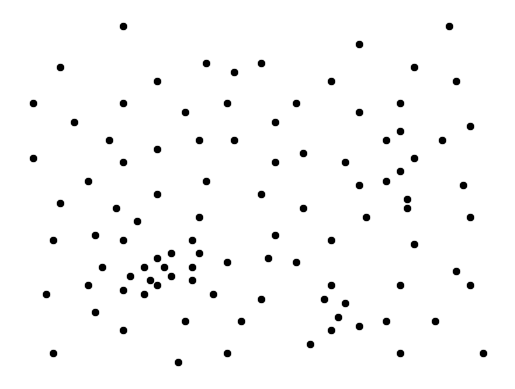
\includegraphics[width=0.3\linewidth]{figures/cls_r.png}}\quad
    \subfloat[Lớp RC]{
\includegraphics[width=0.3\linewidth]{figures/cls_rc.png}}
  \caption{Lớp các cấu hình}
  
  \end{figure}
\end{frame}

\begin{frame}{Thực nghiệm - Phân loại cấu hình}
  \begin{figure}
    \centering
    \subfloat[Lớp C]{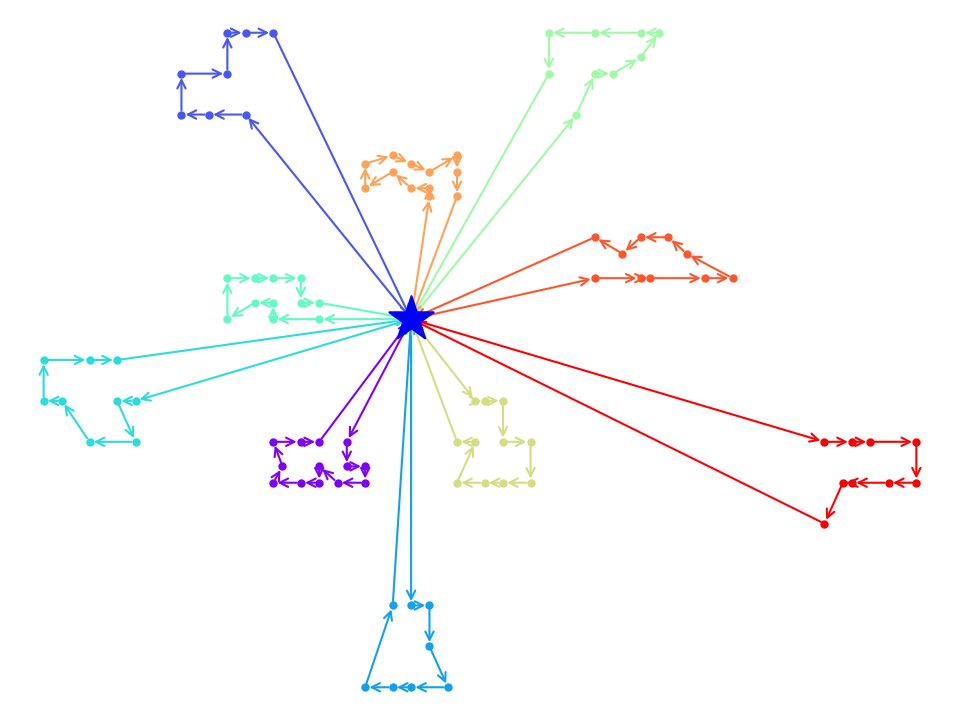
\includegraphics[width=0.3\linewidth]{figures/routes_c101.png}}\quad
    \subfloat[Lớp R]{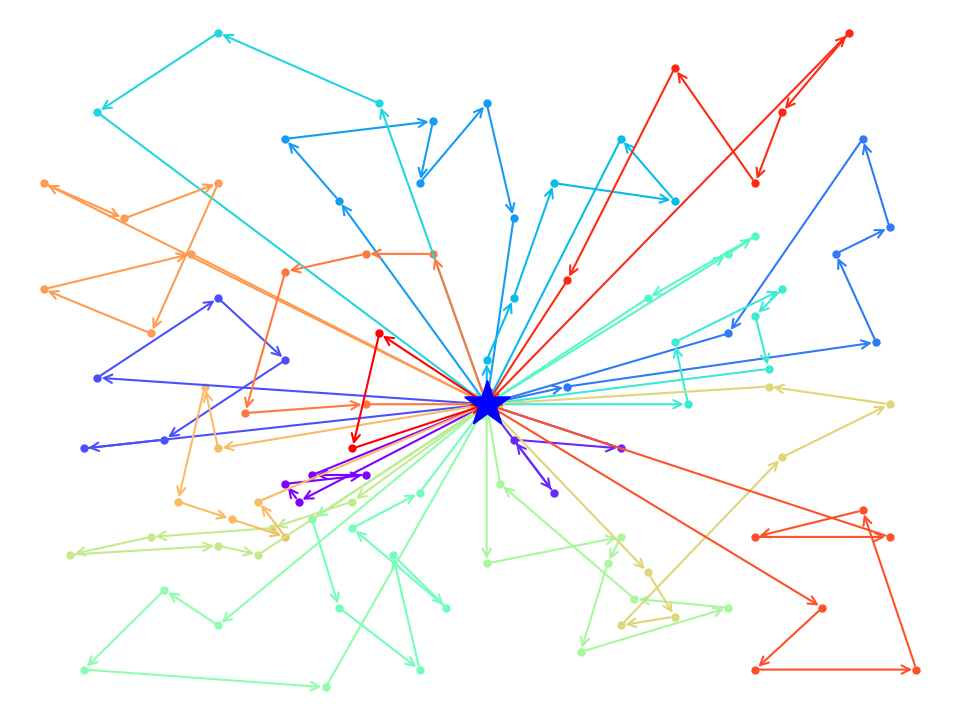
\includegraphics[width=0.3\linewidth]{figures/routes_r101.png}}\quad
    \subfloat[Lớp RC]{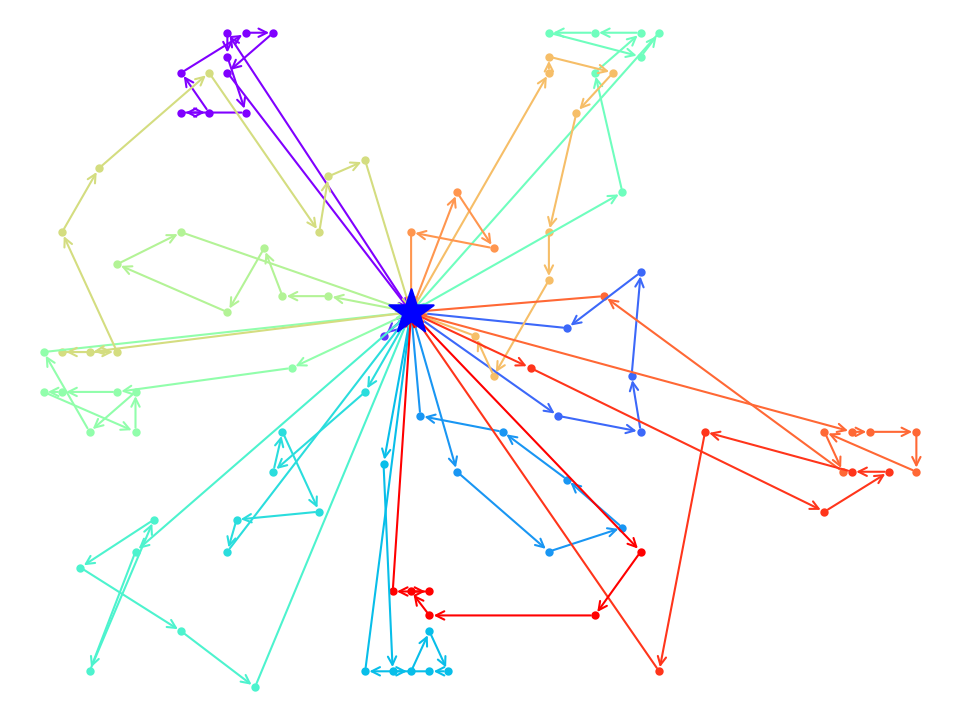
\includegraphics[width=0.3\linewidth]{figures/routes_rc101.png}}
    \caption{Minh họa lời giải cho các lớp cấu hình}
  \end{figure}
\end{frame}

\begin{frame}{Thực nghiệm}
  \begin{block}{Định dạng cấu hình Solomon}
    \begin{itemize}
      \item Tên cấu hình
      \item Số xe được sử dụng
      \item Tải trọng của mỗi xe
      \item ID của yêu cầu
      \item Tọa độ các yêu cầu
      \item Nhu cầu (về tải) của mỗi yêu cầu
      \item Khung thời gian của mỗi yêu cầu
      \item Thời gian phục vụ của mỗi yêu cầu
    \end{itemize}
  \end{block}
\end{frame}

\begin{frame}{Thực nghiệm - Tập Solomon}
  \begin{table}
    \begin{tabular}{|c|c|c|c|}
      \hline
      ins & ALNS & best known & gap (\%) \\ \hline
      c1 & 828.38 & 826.70 & 0.20 \\ \hline
      c2 & 589.86 & 587.38 & 0.42 \\ \hline
      r1 & 1,180.36 & 1,173.61 & 0.61 \\ \hline
      r2 & 883.92 & 872.51 & 1.38 \\ \hline
      rc1 & 1,339.14 & 1,334.49 & 0.36 \\ \hline
      rc2 & 1,007.99 & 1,000.68 & 0.74 \\ \hline
    \end{tabular}
    \caption{Kết quả thực nghiệm trên tập Solomon}
  \end{table}
\end{frame}

\begin{frame}{Thực nghiệm - Tập Solomon}
  \begin{table}
    \small
    \centering
    \begin{tabular}{lrrrll}
    \hline
    instance & alns best & nv & bk cost & bk nv & gap (\%) \\ \hline
    r201 & 1,152.96 & \textbf{7} & 1,143.20 & 8 & 0.32 \\ \hline
    r202 & 1,035.32 & \textbf{7} & 1,029.60 & 8 & 0.42 \\ \hline
    r203 & 880.90 & 6 & 870.80 & 6 & 0.41 \\ \hline
    r204 & 743.91 & \textbf{4} & 731.30 & 5 & 0.53 \\ \hline
    r205 & 958.81 & 5 & 949.80 & 5 & 0.40 \\ \hline
    r206 & 883.92 & 5 & 875.90 & 5 & 0.39 \\ \hline
    r207 & 806.31 & 5 & 794.00 & 4 & 0.85 \\ \hline
    r208 & 948.57 & 4 & 701.00 & 4 & 1.77 \\ \hline
    r209 & 717.53 & 5 & 854.80 & 5 & 0.48 \\ \hline
    r210 & 909.32 & \textbf{5} & 900.50 & 6 & 0.99 \\ \hline
    r211 & 1,053.50 & 5 & 746.70 & 4 & 0.46 \\ \hline
    avg &  &  &  &  & 1.38 \\ \hline
    \end{tabular}
    \caption{Kết quả đo với tập Solomon R2}
    % \end{adjustbox}
  \end{table}
\end{frame}

\begin{frame}{Thực nghiệm - Tập Solomon}
  \begin{table}[, label=exp:solomonRC2, placement=h]
    \small
    \centering
    \begin{tabular}{rrrrrr}
    \hline
    instance & alns best & nv & bk cost & bk nv & gap (\%) \\ \hline
    rc201 & 1,274.61 & \textbf{8} & 1,261.80 & 9 & 1.02 \\ \hline
    rc202 & 1,099.54 & \textbf{6} & 1,092.30 & 8 & 0.66 \\ \hline
    rc203 & 931.16 & 5 & 923.70 & 5 & 0.81 \\ \hline
    rc204 & 788.66 & 4 & 783.50 & 4 & 0.66 \\ \hline
    rc205 & 1,157.66 & 7 & 1,154.00 & 7 & 0.32 \\ \hline
    rc206 & 1,060.50 & \textbf{6} & 1,051.10 & 7 & 0.89 \\ \hline
    rc207 & 966.08 & 6 & 962.90 & 6 & 0.33 \\ \hline
    rc208 & 785.73 & 4 & 776.10 & 4 & 1.24 \\ \hline
    avg &  &  &  &  & 0.74 \\ \hline
    \end{tabular}
    \caption{Kết quả đo với tập Solomon RC2}
    % \end{adjustbox}
  \end{table}
\end{frame}

\begin{frame}{Thực nghiệm - Tập HG}
  \begin{table}
    \begin{tabular}{cccccc}
      \hline
      ins & best & avg & std & bk & gap (\%) \\ \hline
      C1\_2 & 2,679.01 & 2,686.94 & 11.44 & 2,672.73 & 0.23 \\ \hline
      C1\_4 & 7,158.13 & 7,216.72 & 58.54 & 7,021.10 & 1.99 \\ \hline
      C1\_6 & 14,626.95 & 14,867.10 & 202.71 & 13,879.77 & 5.44 \\ \hline
      C1\_8 & 27,131.40 & 27,633.31 & 393.53 & 24,652.04 & 10.11 \\ \hline
      C1\_10 & 47,005.59 & 47,904.60 & 632.61 & 41,232.21 & 14.06 \\ \hline
    \end{tabular}
    \caption{Kết quả thực nghiệm trên tập HG - C1 từ 200 đến 1000 yêu cầu}
  \end{table}
\end{frame}

\begin{frame}{Thực nghiệm - Tập HG}
  \begin{table}
    \begin{tabular}{cccccc}
      \hline
      ins & best & avg & std & bk & gap (\%) \\ \hline
      R1\_2 & 3,628.58 &	3,657.67 &20.33	& 3,572.90	& 1.60 \\ \hline
      R1\_4 & 8,691.74 & 8,767.74 &	56.40	&	8,334.37	& 4.35 \\ \hline
      R1\_6 & 19,079.78 & 19,234.81 & 109.56 & 17,758.66 & 7.47 \\ \hline
      R1\_8 & 34,272.76 &	34,595.79	& 230.14	& 30,959.89	& 10.69 \\ \hline
      R1\_10 & 54,042.04 & 54,636.52 & 376.85	& 46,854.07	& 15.40 \\ \hline
    \end{tabular}
    \caption{Kết quả thực nghiệm trên tập HG - R1 từ 200 đến 1000 yêu cầu}
  \end{table}
\end{frame}

\begin{frame}{Thực nghiệm - Tập HG}
  \begin{table}
    \begin{tabular}{cccccc}
      \hline
      ins & best & avg & std & bk & gap (\%) \\ \hline
      RC1\_2 & 3,205.24	& 3,235.20 & 25.30 & 3,151.30	& 1.73 \\ \hline
      RC1\_4 & 8,304.23 & 8,380.06	& 60.39	& 7,849.98 & 5.78 \\ \hline
      RC1\_6 & 17,185.75 & 17,322.09 & 112.87 & 15,918.08	& 7.98 \\ \hline
      RC1\_8 & 31,245.28 & 31,491.67 & 191.38 & 28,424.05	&	9.91 \\ \hline
      RC1\_10 & 49,633.08	& 50,050.37	& 321.19 & 43,859.18 & 13.15 \\ \hline
    \end{tabular}
    \caption{Kết quả thực nghiệm trên tập HG - RC1 từ 200 đến 1000 yêu cầu}
  \end{table}
\end{frame}

% \begin{frame}{Thực nghiệm - Hiệu năng}
%   \begin{figure}
%     \centering
%     \subfloat[60s]{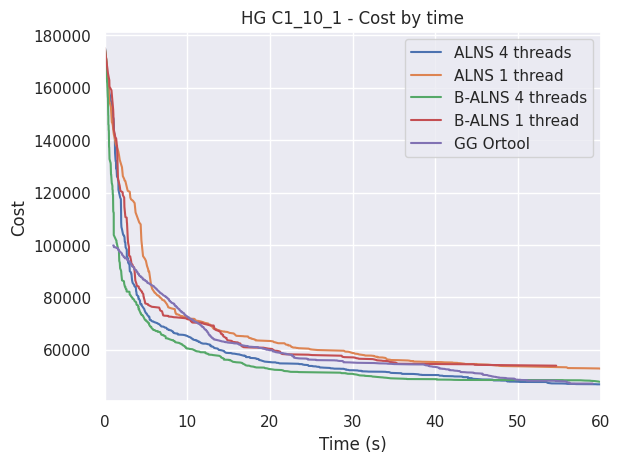
\includegraphics[width=0.4\linewidth]{figures/cost_time_60s_C1_10_1.png}}\quad
%     \subfloat[10s]{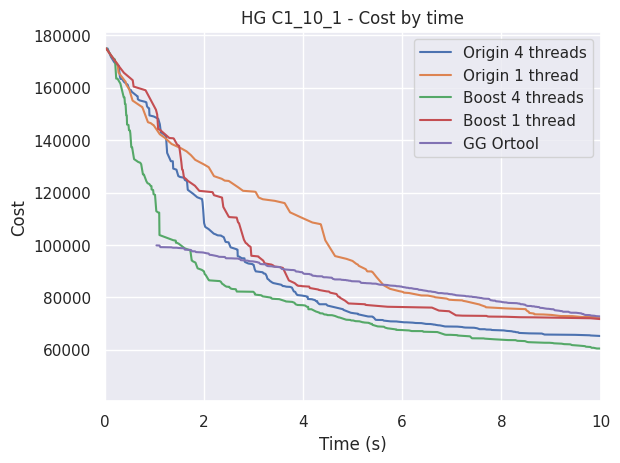
\includegraphics[width=0.4\linewidth]{figures/cost_time_10s_C1_10_1.png}}
%   \caption{Giá trị hàm mục tiêu theo thời gian, cấu hình C1\_10\_1}
%   \end{figure}
% \end{frame}

\begin{frame}{Thực nghiệm - Hiệu năng}
  \begin{figure}
    \centering
    \subfloat[60s]{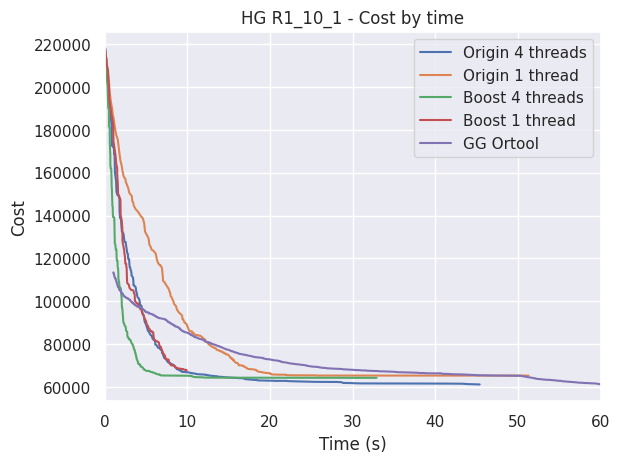
\includegraphics[width=0.4\linewidth]{figures/cost_time_60s_R1_10_1.png}}\quad
    \subfloat[10s]{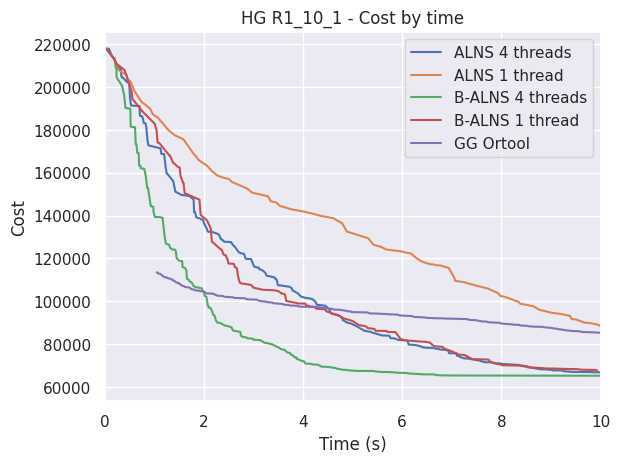
\includegraphics[width=0.4\linewidth]{figures/cost_time_10s_R1_10_1.png}}
  \caption{Giá trị hàm mục tiêu theo thời gian, cấu hình R1\_10\_1}
  \end{figure}
\end{frame}

% \begin{frame}{Thực nghiệm - Hiệu năng}
%   \begin{figure}
%     \centering
%     \subfloat[60s]{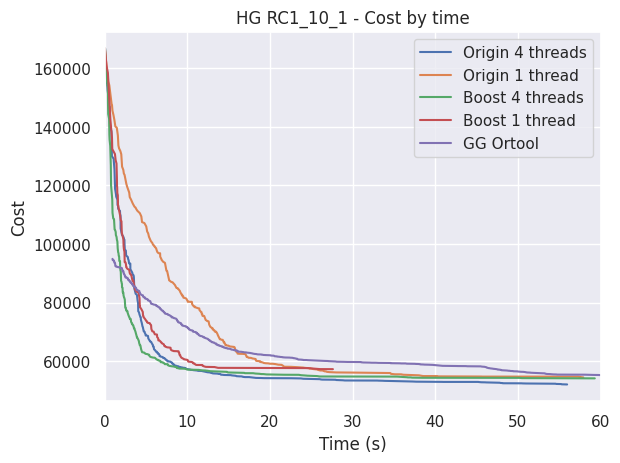
\includegraphics[width=0.4\linewidth]{figures/cost_time_60s_RC1_10_1.png}}\quad
%     \subfloat[10s]{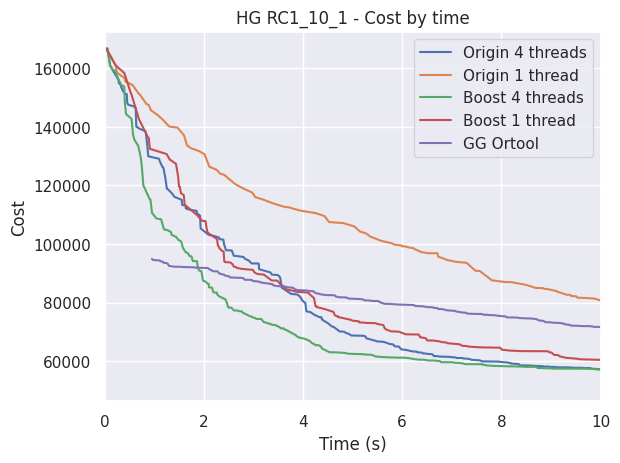
\includegraphics[width=0.4\linewidth]{figures/cost_time_10s_RC1_10_1.png}}
%   \caption{Giá trị hàm mục tiêu theo thời gian, cấu hình RC1\_10\_1}
%   \end{figure}
% \end{frame}

% \begin{frame}{Thực nghiệm - Hiệu năng}
%   \begin{figure}
%     \centering
%     \subfloat[10s]{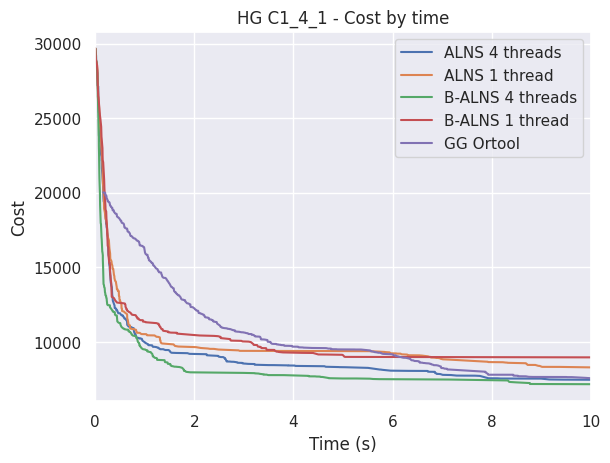
\includegraphics[width=0.4\linewidth]{figures/cost_time_10s_C1_4_1.png}}\quad
%     \subfloat[1s]{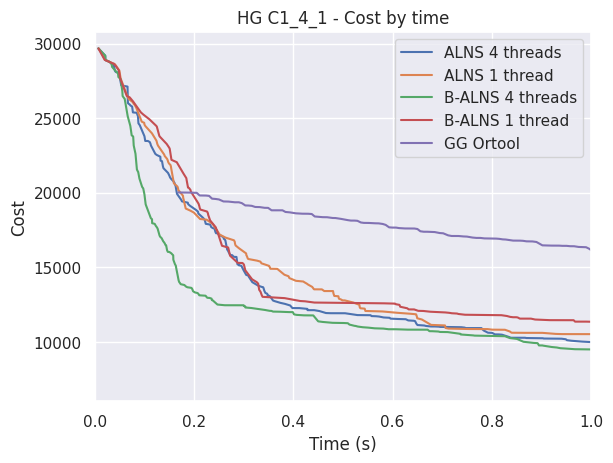
\includegraphics[width=0.4\linewidth]{figures/cost_time_1s_C1_4_1.png}}
%   \caption{Giá trị hàm mục tiêu theo thời gian, cấu hình C1\_4\_1}
%   \end{figure}
% \end{frame}

% \begin{frame}{Thực nghiệm - Hiệu năng}
%   \begin{figure}
%     \centering
%     \subfloat[10s]{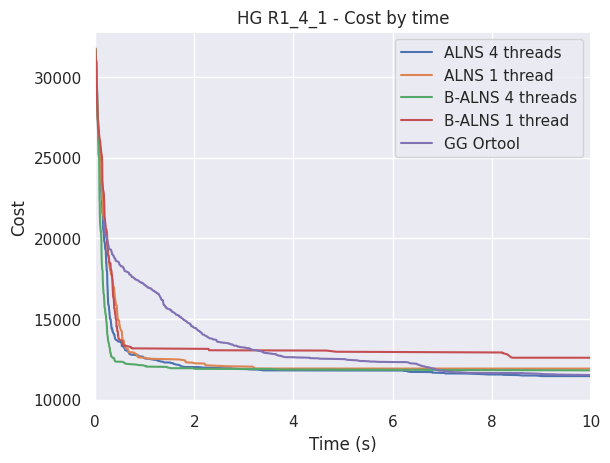
\includegraphics[width=0.4\linewidth]{figures/cost_time_10s_R1_4_1.png}}\quad
%     \subfloat[1s]{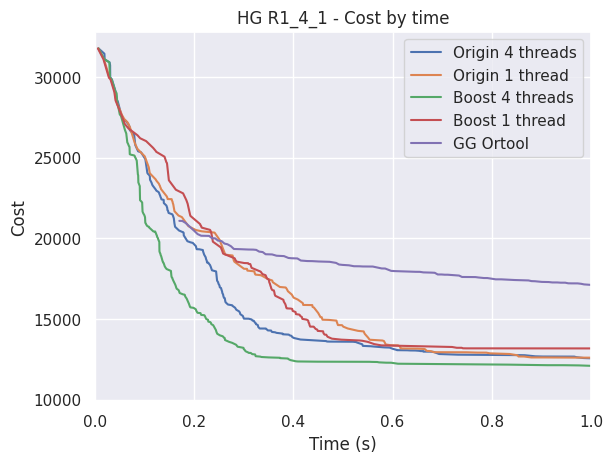
\includegraphics[width=0.4\linewidth]{figures/cost_time_1s_R1_4_1.png}}
%   \caption{Giá trị hàm mục tiêu theo thời gian, cấu hình R1\_4\_1}
%   \end{figure}
% \end{frame}

\begin{frame}{Thực nghiệm - Hiệu năng}
  \begin{figure}
    \centering
    \subfloat[10s]{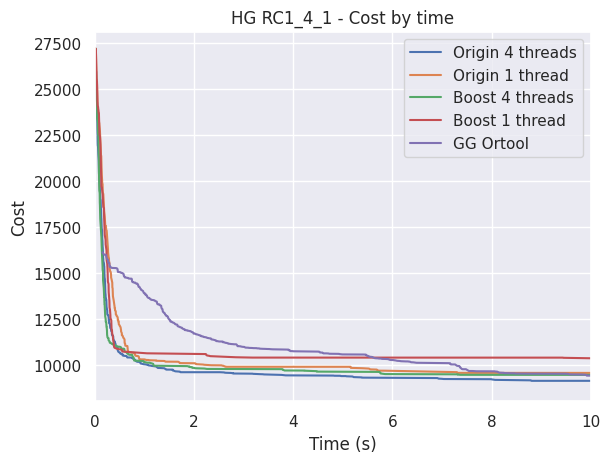
\includegraphics[width=0.4\linewidth]{figures/cost_time_10s_RC1_4_1.png}}\quad
    \subfloat[1s]{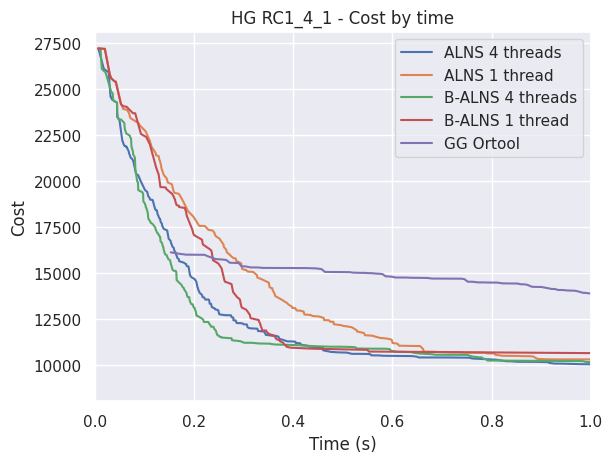
\includegraphics[width=0.4\linewidth]{figures/cost_time_1s_RC1_4_1.png}}
  \caption{Giá trị hàm mục tiêu theo thời gian, cấu hình RC1\_4\_1}
  \end{figure}
\end{frame}

% \begin{frame}{Thực nghiệm - Hiệu năng}
%   \begin{figure}
%     \centering
%     \subfloat[60s]{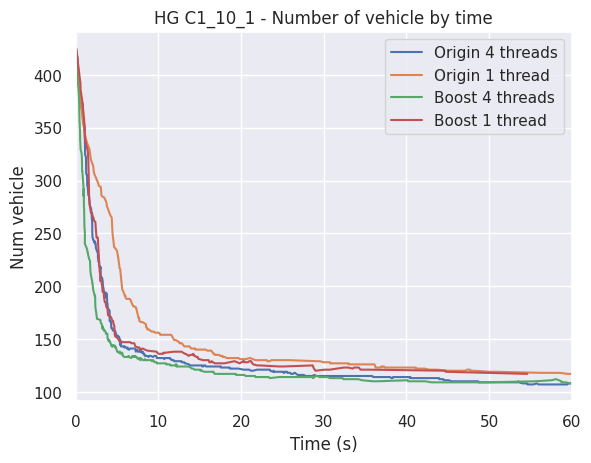
\includegraphics[width=0.4\linewidth]{figures/nv_time_60s_C1_10_1.png}}\quad
%     \subfloat[10s]{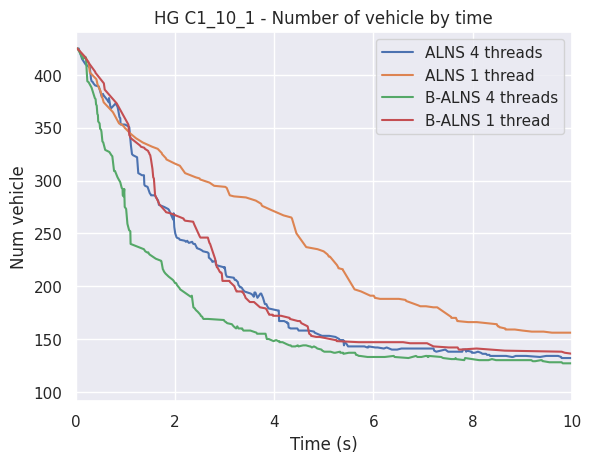
\includegraphics[width=0.4\linewidth]{figures/nv_time_10s_C1_10_1.png}}
%   \caption{Số xe sử dụng theo thời gian, cấu hình C1\_10\_1}
%   \end{figure}
% \end{frame}

\begin{frame}{Thực nghiệm - Hiệu năng}
  \begin{figure}
    \centering
    \subfloat[60s]{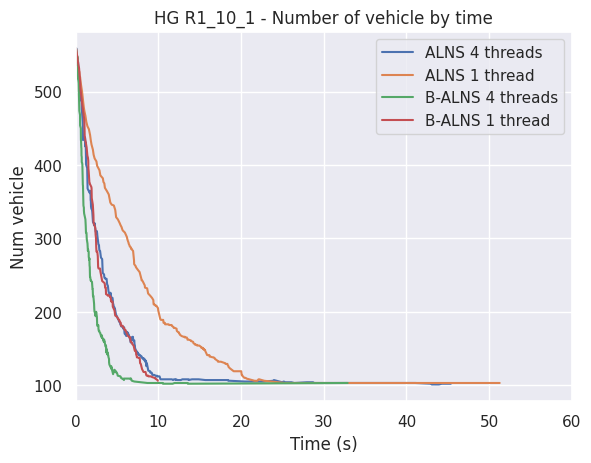
\includegraphics[width=0.4\linewidth]{figures/nv_time_60s_R1_10_1.png}}\quad
    \subfloat[10s]{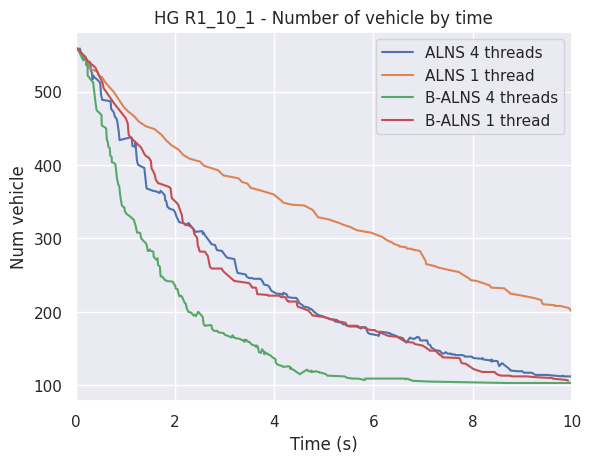
\includegraphics[width=0.4\linewidth]{figures/nv_time_10s_R1_10_1.png}}
  \caption{Số xe sử dụng theo thời gian, cấu hình R1\_10\_1}
  \end{figure}
\end{frame}

% \begin{frame}{Thực nghiệm - Hiệu năng}
%   \begin{figure}
%     \centering
%     \subfloat[60s]{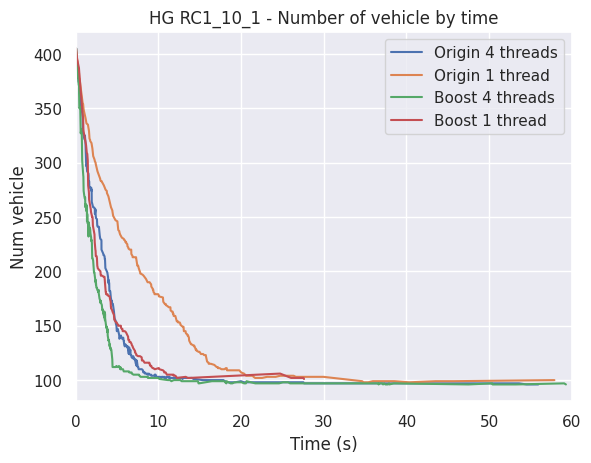
\includegraphics[width=0.4\linewidth]{figures/nv_time_60s_RC1_10_1.png}}\quad
%     \subfloat[10s]{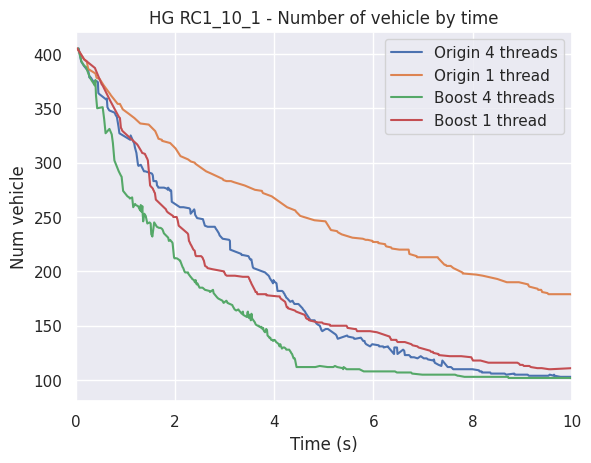
\includegraphics[width=0.4\linewidth]{figures/nv_time_10s_RC1_10_1.png}}
%   \caption{Số xe sử dụng theo thời gian, cấu hình RC1\_10\_1}
%   \end{figure}
% \end{frame}

% \begin{frame}{Thực nghiệm - Hiệu năng}
%   \begin{figure}
%     \centering
%     \subfloat[10s]{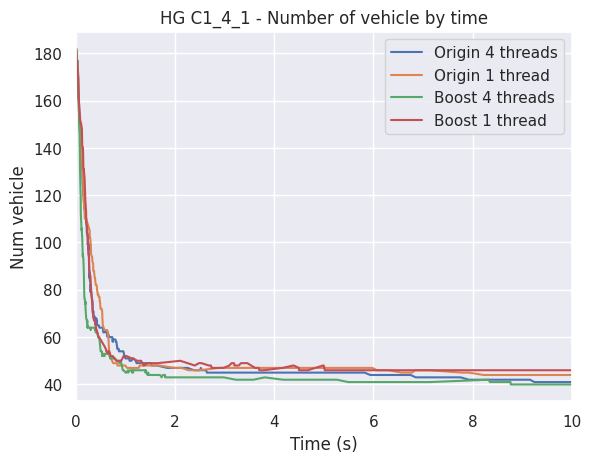
\includegraphics[width=0.4\linewidth]{figures/nv_time_10s_C1_4_1.png}}\quad
%     \subfloat[1s]{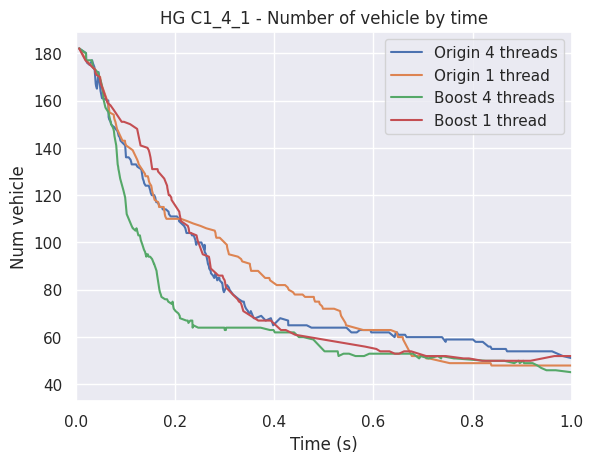
\includegraphics[width=0.4\linewidth]{figures/nv_time_1s_C1_4_1.png}}
%   \caption{Số xe sử dụng theo thời gian, cấu hình C1\_4\_1}
%   \end{figure}
% \end{frame}

\begin{frame}{Thực nghiệm - Hiệu năng}
  \begin{figure}
    \centering
    \subfloat[10s]{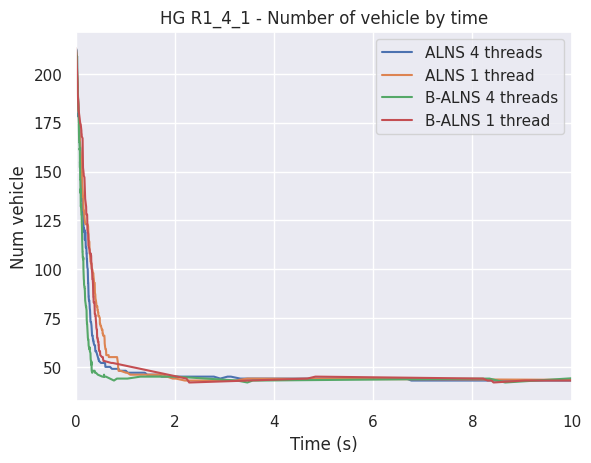
\includegraphics[width=0.4\linewidth]{figures/nv_time_10s_R1_4_1.png}}\quad
    \subfloat[1s]{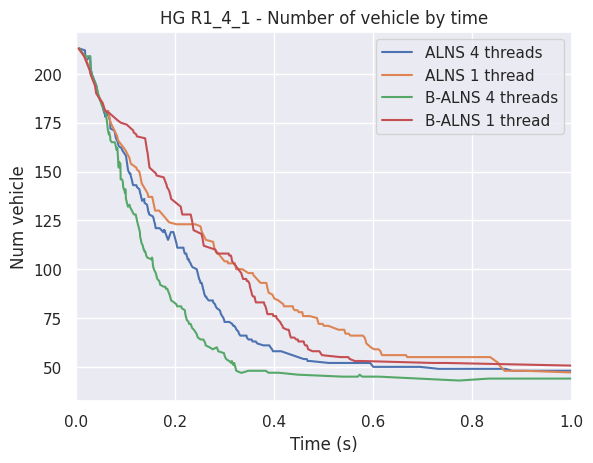
\includegraphics[width=0.4\linewidth]{figures/nv_time_1s_R1_4_1.png}}
  \caption{Số xe sử dụng theo thời gian, cấu hình R1\_4\_1}
  \end{figure}
\end{frame}

% \begin{frame}{Thực nghiệm - Hiệu năng}
%   \begin{figure}
%     \centering
%     \subfloat[10s]{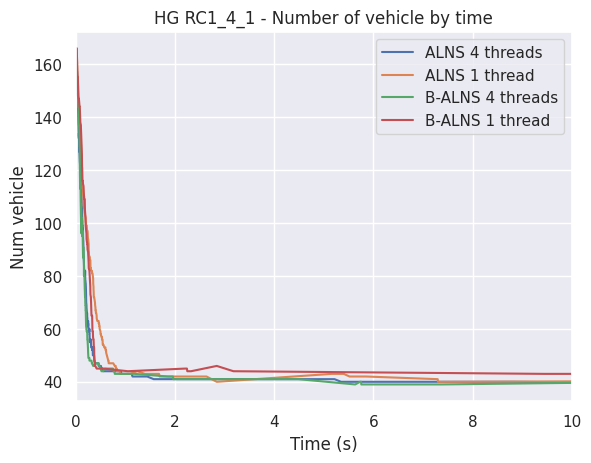
\includegraphics[width=0.4\linewidth]{figures/nv_time_10s_RC1_4_1.png}}\quad
%     \subfloat[1s]{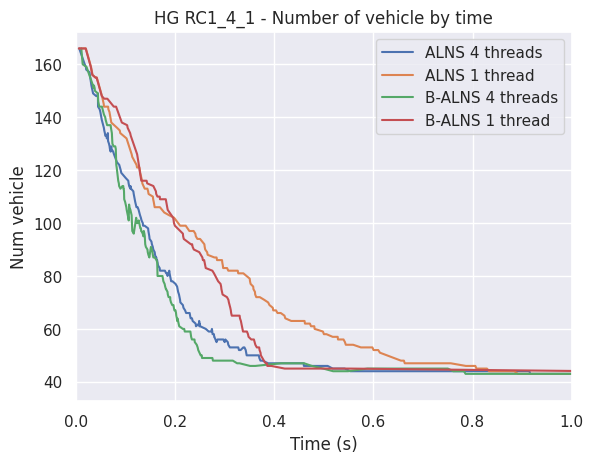
\includegraphics[width=0.4\linewidth]{figures/nv_time_1s_RC1_4_1.png}}
%   \caption{Số xe sử dụng theo thời gian, cấu hình RC1\_4\_1}
%   \end{figure}
% \end{frame}

\begin{frame}{Thực nghiệm - Thuật toán hủy}
  \begin{figure}[H] % places figure environment here   
    \centering % Centers Graphic
    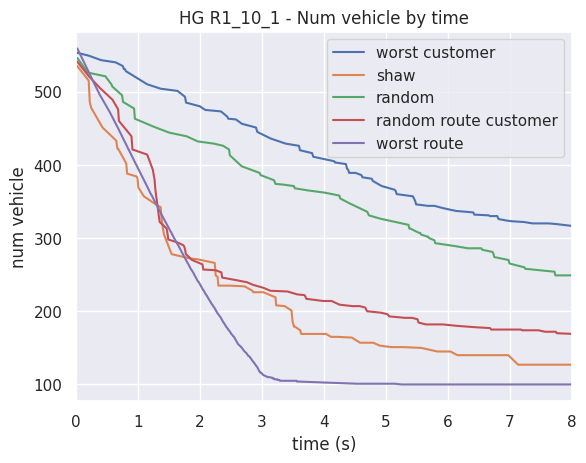
\includegraphics[width=0.6\textwidth]{figures/nv_time_des_10s_R1_10_1.png}
    % \includesvg[scale=1]{figures/core-object}
    \caption{Số xe theo thời gian với các thuật toán hủy khác nhau}
    \label{fig:nv_des_01}
  \end{figure}
\end{frame}

\begin{frame}{Thực nghiệm - Tần suất sử dụng thuật toán hủy}
  \begin{figure}[H] % places figure environment here   
    \centering % Centers Graphic
    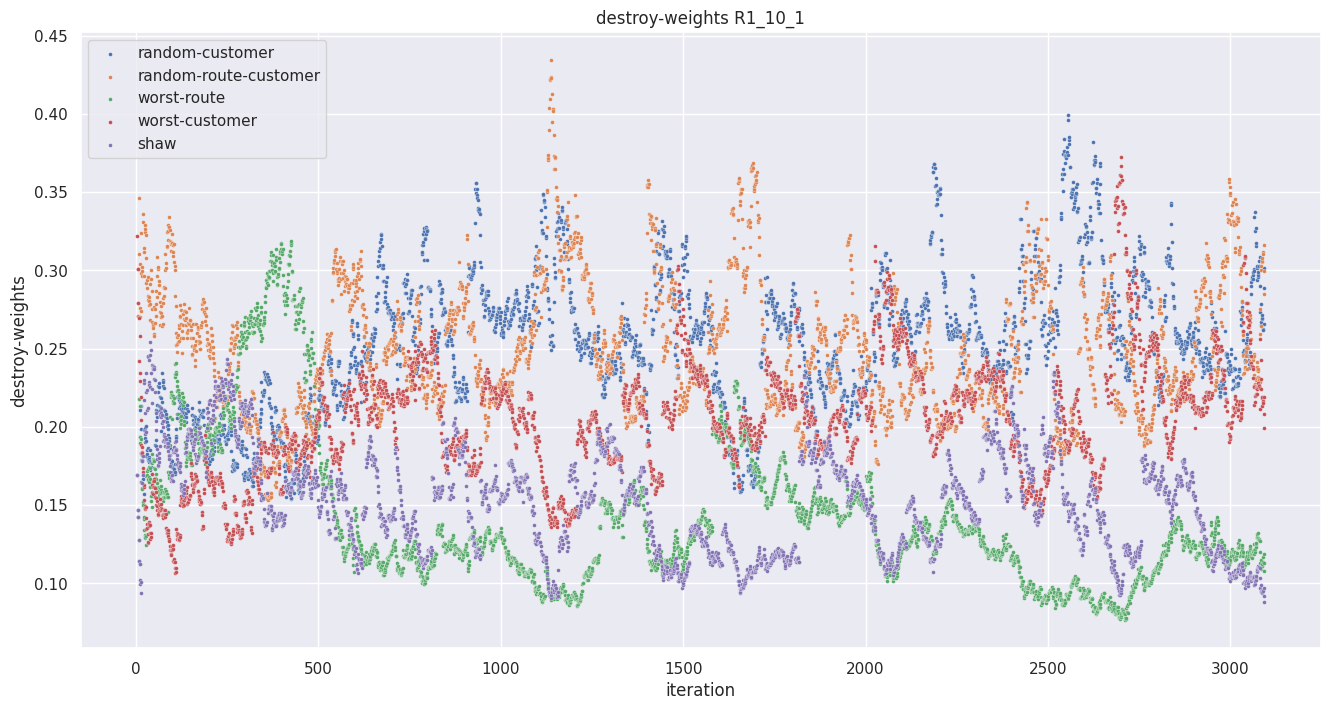
\includegraphics[width=1\textwidth]{figures/destroy_weights_R1_10_1.png}
    % \includesvg[scale=1]{figures/core-object}
    \caption{Trọng số của các thuật toán hủy}
    \label{fig:alg_01}
  \end{figure}
\end{frame}

\begin{frame}{Thực nghiệm - Tần suất sử dụng thuật toán chèn}
  \begin{figure}[H] % places figure environment here   
    \centering % Centers Graphic
    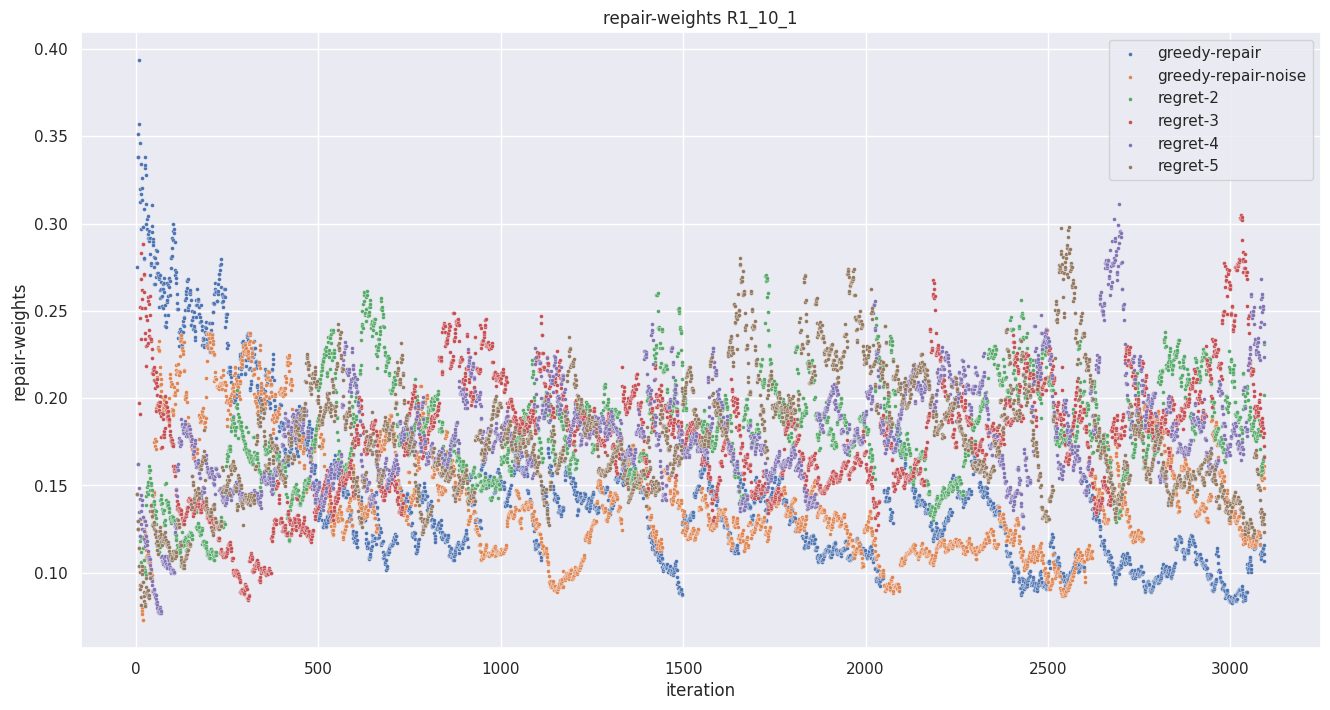
\includegraphics[width=1\textwidth]{figures/repair_weights_R1_10_1.png}
    % \includesvg[scale=1]{figures/core-object}
    \caption{Trọng số của các thuật toán chèn}
    \label{fig:alg_02}
  \end{figure}
\end{frame}